\usetikzlibrary{calc}


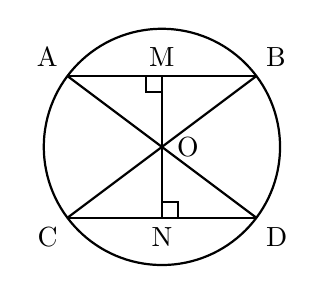
\begin{tikzpicture}[scale=1]

    % Define the center of the circle
    \coordinate (O) at (0,0);

    % Draw the circle
    \draw[thick] (O) circle (1.5);

    % Define coordinates for the points on the circle and chords
    % AB is the top horizontal chord
    \coordinate (A) at (-1.2, 0.9);
    \coordinate (B) at (1.2, 0.9);
    
    % CD is the bottom horizontal chord
    \coordinate (C) at (-1.2, -0.9);
    \coordinate (D) at (1.2, -0.9);

    % M is the midpoint of AB
    \coordinate (M) at (0, 0.9);
    
    % N is the midpoint of CD
    \coordinate (N) at (0, -0.9);

    % Draw the chords AB and CD
    \draw[thick] (A) -- (B);
    \draw[thick] (C) -- (D);

    % Draw the diagonal lines passing through the center O
    \draw[thick] (A) -- (D);
    \draw[thick] (B) -- (C);

    % Draw the vertical line connecting M, O, and N
    \draw[thick] (M) -- (N);

    % Draw the right-angle symbols
    % At M (on the left side)
    \draw[thick] (M) ++(-0.2,0) -- ++(0,-0.2) -- ++(0.2,0);
    % At N (on the right side)
    \draw[thick] (N) ++(0,0.2) -- ++(0.2,0) -- ++(0,-0.2);

    % Add labels for the vertices and midpoints
    \node[above left] at (A) {A};
    \node[above right] at (B) {B};
    \node[below left] at (C) {C};
    \node[below right] at (D) {D};
    
    \node[above] at (M) {M};
    \node[below] at (N) {N};
    
    % Add label for the center O, shifted slightly to avoid overlap with lines
    \node[right, xshift=2pt] at (O) {O};

\end{tikzpicture}